\documentclass[journal,12pt,twocolumn]{IEEEtran}

\usepackage{setspace}
%\usepackage{gensymb}
\singlespacing
\usepackage[cmex10]{amsmath}

\usepackage{amsthm}

\usepackage{mathrsfs}
\usepackage{txfonts}
\usepackage{stfloats}
\usepackage{bm}
\usepackage{cite}
\usepackage{cases}
\usepackage{subfig}
\usepackage{float}
\usepackage{longtable}
\usepackage{multirow}

\usepackage{enumitem}
\usepackage{mathtools}
\usepackage{steinmetz}
\usepackage{tikz}
%\usepackage{circuitikz}
\usepackage{verbatim}
\usepackage{tfrupee}
\usepackage[breaklinks=true]{hyperref}
\usepackage{graphicx}
\usepackage{tkz-euclide}

\usetikzlibrary{calc,math}
\usepackage{listings}
    \usepackage{color}                                            %%
    \usepackage{array}                                            %%
    \usepackage{longtable}                                        %%
    \usepackage{calc}                                             %%
    \usepackage{multirow}                                         %%
    \usepackage{hhline}                                           %%
    \usepackage{ifthen}                                           %%
    \usepackage{lscape}     
\usepackage{multicol}
\usepackage{chngcntr}

\DeclareMathOperator*{\Res}{Res}

\renewcommand\thesection{\arabic{section}}
\renewcommand\thesubsection{\thesection.\arabic{subsection}}
\renewcommand\thesubsubsection{\thesubsection.\arabic{subsubsection}}

\renewcommand\thesectiondis{\arabic{section}}
\renewcommand\thesubsectiondis{\thesectiondis.\arabic{subsection}}
\renewcommand\thesubsubsectiondis{\thesubsectiondis.\arabic{subsubsection}}


\hyphenation{op-tical net-works semi-conduc-tor}
\def\inputGnumericTable{}                                 %%

\lstset{
%language=C,
frame=single, 
breaklines=true,
columns=fullflexible
}
\begin{document}


\newtheorem{theorem}{Theorem}[section]
\newtheorem{problem}{Problem}
\newtheorem{proposition}{Proposition}[section]
\newtheorem{lemma}{Lemma}[section]
\newtheorem{corollary}[theorem]{Corollary}
\newtheorem{example}{Example}[section]
\newtheorem{definition}[problem]{Definition}

\newcommand{\BEQA}{\begin{eqnarray}}
\newcommand{\EEQA}{\end{eqnarray}}
\newcommand{\define}{\stackrel{\triangle}{=}}
\bibliographystyle{IEEEtran}
\raggedbottom
\setlength{\parindent}{0pt}
\providecommand{\mbf}{\mathbf}
\providecommand{\pr}[1]{\ensuremath{\Pr\left(#1\right)}}
\providecommand{\qfunc}[1]{\ensuremath{Q\left(#1\right)}}
\providecommand{\sbrak}[1]{\ensuremath{{}\left[#1\right]}}
\providecommand{\lsbrak}[1]{\ensuremath{{}\left[#1\right.}}
\providecommand{\rsbrak}[1]{\ensuremath{{}\left.#1\right]}}
\providecommand{\brak}[1]{\ensuremath{\left(#1\right)}}
\providecommand{\lbrak}[1]{\ensuremath{\left(#1\right.}}
\providecommand{\rbrak}[1]{\ensuremath{\left.#1\right)}}
\providecommand{\cbrak}[1]{\ensuremath{\left\{#1\right\}}}
\providecommand{\lcbrak}[1]{\ensuremath{\left\{#1\right.}}
\providecommand{\rcbrak}[1]{\ensuremath{\left.#1\right\}}}
\theoremstyle{remark}
\newtheorem{rem}{Remark}
\newcommand{\sgn}{\mathop{\mathrm{sgn}}}
\providecommand{\abs}[1]{(\vert#1)\vert}
\providecommand{\res}[1]{\Res\displaylimits_{#1}} 
\providecommand{\norm}[1]{(\lVert#1)\rVert}
%\providecommand{\norm}[1]{\lVert#1\rVert}
\providecommand{\mtx}[1]{\mathbf{#1}}
\providecommand{\mean}[1]{E([ #1 )]}
\providecommand{\fourier}{\overset{\mathcal{F}}{ \rightleftharpoons}}
%\providecommand{\hilbert}{\overset{\mathcal{H}}{ \rightleftharpoons}}
\providecommand{\system}{\overset{\mathcal{H}}{ \longleftrightarrow}}
	%\newcommand{\solution}[2]{\textbf{Solution:}{#1}}
\newcommand{\solution}{\noindent \textbf{Solution: }}
\newcommand{\cosec}{\,\text{cosec}\,}
\newcommand{\Prod}{\prod\limits}
\providecommand{\dec}[2]{\ensuremath{\overset{#1}{\underset{#2}{\gtrless}}}}
\newcommand{\myvec}[1]{\ensuremath{\begin{pmatrix}#1\end{pmatrix}}}
\newcommand{\mydet}[1]{\ensuremath{\begin{vmatrix}#1\end{vmatrix}}}
\numberwithin{equation}{subsection}
\makeatletter
\@addtoreset{figure}{problem}
\makeatother
\let\StandardTheFigure\thefigure
\let\vec\mathbf
\renewcommand{\thefigure}{\theproblem}
\def\putbox#1#2#3{\makebox[0in][l]{\makebox[#1][l]{}\raisebox{\baselineskip}[0in][0in]{\raisebox{#2}[0in][0in]{#3}}}}
     \def\rightbox#1{\makebox[0in][r]{#1}}
     \def\centbox#1{\makebox[0in]{#1}}
     \def\topbox#1{\raisebox{-\baselineskip}[0in][0in]{#1}}
     \def\midbox#1{\raisebox{-0.5\baselineskip}[0in][0in]{#1}}
\vspace{3cm}
\title{Assignment 4}
\author{Taha Adeel Mohammed - CS20BTECH11052}
\maketitle
\newpage
\bigskip
\renewcommand{\thefigure}{\theenumi}
\renewcommand{\thetable}{\theenumi}
Download all python codes from 
\begin{lstlisting}
https://github.com/Taha-Adeel/AI1103/tree/main/Assignment_4/Codes
\end{lstlisting}
%
and latex-tikz codes from 
%
\begin{lstlisting}
https://github.com/Taha-Adeel/AI1103/tree/main/Assignment_4
\end{lstlisting}
\section{Problem (GATE 2021 (ST) Q.19)}
%%(GATE 2021 (ST) Q.19 ( statistics section)) \\
Let $\{ X_n \}_{n \geq 1}$ be a sequence of independent and identically distributed random variables each having uniform distribution on (0,2). For $n \geq 1$, let 
$$Z_n = -\log_e \left( \Prod_{i=1}^n (2-X_i) \right)^\frac{1}{n}.
$$
Then, as $n \to \infty$, the sequence $\{ Z_n \}_{n \geq 1}$ converges almost surely to \rule{1cm}{0.15mm} (Round of to 2 decimal places).
\section{Solution (GATE 2021 (ST) Q.19)}
Simplifying $Z_n$, we have
\begin{align}
    Z_n &= -\log_e \left( \Prod_{i=1}^n (2-X_i) \right)^\frac{1}{n}\\
        &= -\frac{1}{n}\cdot \log_e \left( \Prod_{i=1}^n (2-X_i) \right)\\
        &= \frac{1}{n}\cdot\left( \sum\limits_{i=1}^n (-\log_e \left( 2-X_i )\right) \right)
\end{align}
Let $X$ and $Z$ be random variables. $X$ follows a uniform distribution from 0 to 2.
\begin{align}
    X &\sim \mathcal{U}[0,2],\\
    \text{and let }    Z&=-\log_e (2-X)
\end{align}
In our question, we are generating $n$ independent and identically distributed random variables, $X_i , \text{where } i \leq n$ from $X \sim \mathcal{U}[0,2]$ and $Z_n$ finds the average value of $-\log_e (2-X_i)$ . \textbf{The Law of Large Numbers} states that for large number of trials($n$ here), the average obtained (of $-\log_e (2-X_i)$ here) should be close to the expected value (of $-\log_e (2-X)=E(Z)$ here), and will tend to become closer to the expected value as more trials are performed.. Hence as $n \to \infty$, the sequence $\{Z_n\} $ tends to the expectation value of the continuous distribution of $Z$.
\begin{align}
    \therefore \lim\limits_{n \to \infty}Z_n&=E(Z)
    \label{Zn_and_Z}
\end{align}
The CDF of $Z$ is defined as 
\begin{align}
    F_Z(z) &= \pr{Z \leq z} \\
           &= \pr{ -\log_e(2-X)\leq z} \\
           &= \pr{\log_e(2-X) \geq -z}\\
           &= \pr{2-X \geq \exp\brak{-z}}\\
           &= \pr{X \leq 2- \exp\brak{-z}}\\
           &= F_X\brak{2- \exp\brak{-z}}
%           \\&=  1-\frac{exp(-z)}{2}
\label{CDF_Z}
\end{align}
The CDF for X ($F_X(x)$), a uniform distribution on $(0,2)$ is given by
\begin{align}
F_X(x) = 
\begin{cases}
0 &  x < 0 \\
\frac{x}{2} & 0 \leq x \leq 2 \\
1 & x > 2
\end{cases}
\end{align}
%
Substituting the above in \eqref{CDF_Z},
%
\begin{multline}
F_X\brak{2- \exp(-z)} =
\\
\begin{cases}
0 &  2- \exp(-z) < 0 \\
1- \frac{\exp(-z)}{2} & 0 \leq 2- \exp(-z) \leq 2 \\
1 & 2- \exp(-z) > 2
\end{cases}
\end{multline}
After some algebra, the above conditions yield
\begin{align}
F_Z(z) &= 
\begin{cases}
0 & z < -\log_e (2) \\
1- \frac{\exp(-z)}{2} & z \geq -\log_e (2)
\end{cases}
\label{CDF_Z_Final}\\
\implies f_Z(z)&=\dfrac{\text{d}(F_Z(z))}{\text{d}z}   
=\begin{cases}
0 & z < -\log_e (2) \\
\frac{\exp(-z)}{2} & z \geq -\log_e (2)
\end{cases}
\label{PDF_Z_Final}
\end{align}
\begin{figure}[H]
    \centering
      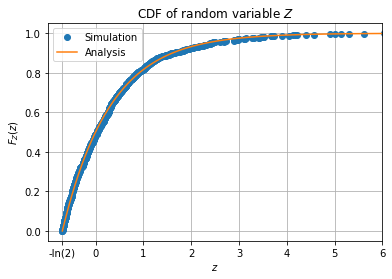
\includegraphics[width=\columnwidth]{Figures/CDF_Z.png}
     \caption{$F_Z(z)$}
\end{figure}
Now calculating the expectation value for $Z$, we have
\begin{align}
    E(Z)&=\int\limits_{-\ln{2}}^{\infty}z\,f_Z(z)\,dz\\
    &=\int\limits_{-\ln{2}}^{\infty}\dfrac{z\,e^{-z}}{2}\,dz\\
    &=\left[ \dfrac{-(z+1)\,e^{-z}}{2} \right]_{-\ln{2}}^\infty\\
    &=1-\ln{(2)}\\
    &\approx0.3068
\end{align}
\par From \eqref{Zn_and_Z}, we have as $n \to \infty$, $Z_n \to E(Z)=0.3068\approx0.31$(Rounded to 2 decimal places).\\
\textbf{Ans: 0.31}
\end{document}
